%
% 計測自動制御学会システム・情報部門学術講演会2013原稿サンプルファイル
%                                           August 26, 2013
% 計測自動制御学会システム・情報部門学術講演会2011原稿サンプルファイル
%                                           April 28, 2011
% Based on 第7回計測自動制御学会制御部門大会原稿サンプルファイル
%                                           October 18, 2007
% Based on 第5回計測自動制御学会制御部門大会原稿サンプルファイル
%            近野敦 konno@space.mech.tohoku.ac.jp    March 05, 2005
%
% LaTeX2eとLaTeX209判別のための定義(以下3行)は科研費マクロkkhgrp.mac
% の定義を,作者の金沢大学青木先生の許可を得て利用させていただきました.
%
\newif\ifLaTeXe\LaTeXefalse
\expandafter\ifx\csname PackageError\endcsname\relax\LaTeXefalse
\else\LaTeXetrue\fi

\ifLaTeXe
  \documentclass{jarticle}
  \usepackage{SICE-SSI}
  \usepackage[dvipdfmx]{graphicx}
  \usepackage{multicol}
 % \usepackage{utf8}{inputenc}
 % \usepackage{otf}
  %\DeclareUnicodeCharacter{9AD9}{\UTF{9AD9}} % 髙
%  \usepackage{tabularx}
\else
  \documentstyle[SICE-SSI,epsbox]{jarticle}
\fi

\begin{document}
\title{複数解探索を考慮した分散型Bat Algorithm}
\author{○岩瀬拓哉\ \ 高野諒\ \ 上野史\ \ 梅内祐太\ \ 石井晴之\ \ \ 佐藤寛之\ \ 高玉圭樹\ (電気通信大学)}

\abstract{
近年,最適解問題に対する大域的探索手法としてBat Algorithmが提案され様々な研究がなされている.
しかし,Bat Algotithmは解を更新する際に過去に探索した最良解を参照する探索特性をもつため,最終的に最適解付近に収束してしまい複数の局所解を同時に探索することが困難である.
そこで,複数の局所解の同時探索を可能にするため2つの修正を加えた分散型Bat Algorithmを提案する.具体的な修正点は以下の2点である.(1)各個体間の距離を考慮した速度の更新;(2)新たな解の生成時に各個体の最良解(パーソナルベスト)に基づく新たな解の生成.
複数の局所解をもつ多峰性ベンチマーク問題を用いたシミュレーション実験により提案手法の複数の局所解の網羅的な探索性能の有効性を検証する.
その結果,上記の修正を加えることによって従来のBAと比較して分散BAがより多くの局所解を探索しており,修正が複数の局所解の網羅的な探索に対して有効であることを示した.
}

\keyword{Meta-Heuristics, Bat Algorithm, Optimization Problem}

\maketitle\thispagestyle{empty}
\pagestyle{empty}

\section{はじめに}

%大域的な探索が可能なメタヒューリスティック手法には,魚や鳥といった群れを成す動物の行動をモデル化した粒子群最適化(Particle Swarm Opti-mization: PSO)\cite{1}やホタルの光強度によって明るいホタルの方へ他のホタルが惹きよせられる特性を利用したFA(Firefly Algorithm)\cite{2}が例として挙げられる.中でもYangが提案したBat Algorithm(以下,BA)\cite{3}は,コウモリの特性であるエコロケーションを用いて対象物に向かって周波数を発し,その反射波から対象物との距離を計測し,周囲の状況を知るという特性に着想を得て設計されたアルゴリズムである.BAは本研究では,不特定多数の被災者の探索を行う救助ロボットへの適用を想定して,BAにおけるコウモリ特有の周波数を用いて確率的な行動を抑制し,複数解探索性能の向上を図る.特に,災害時での不特定多数の各被災者を多峰性関数における複数の局所解と見立て,シミュレーション実験にて性能の検証を行った.

Bat Algotithm(BA)はコウモリが獲物や障害物の距離を測定するために用いるエコーロケーションという行動に着想を得て設計された多点探索型アルゴリズムである.\cite{1}
BAは他の多点探索アルゴリズムである魚や鳥の群れをモデル化した粒子群最適化(Particle Swarm Optimization:PSO)\cite{2}や
光強度によって他の個体を引き寄せるホタルの特性に着想を得たFirefly Algorithm(FA)\cite{3}や様々な問題に対応させた(FA Searching Multiple Solutions:MSFA)\cite{4}などと同様に多峰性を持つ高次元の最適化問題において優良な探索性能を持つことが知られている.
BAは解の探索において各個体が過去に探索した最優良解を参照し探索するため,最終的に全個体が最適解付近に収束してしまう.
しかし,現実世界の問題への応用を考えたとき,災害時の要救助者の探索において被災者の数や,その状態による優先度を考慮するように,最適解のみではなくその他の優良な局所解の探索が求められる場合がある.
他の多点探索アルゴリズムに基づく複数の局所解の探索を考慮した手法として,人工蜂コロニーアルゴリズム(Artificial Bee Colony Algorithm:ABC)に基づいたABC-lis\cite{5}などが提案されているが,
BAに基づいた複数の局所解の探索を考慮した修正については多くの研究がなされていない.
そこで本研究では,従来のBAに対して複数の局所解の網羅的な探索性能向上のために2つの修正を加えた分散型Bat Algorithm(分散BA)を提案する.
具体的な修正点は以下の2つである:
(1)各世代において各個体間の距離を考慮した速度の更新;
(2)新たな解の生成時に各個体の最良解(パーソナルベスト)を参照した解の生成.
提案手法である分散BAの複数の局所解の網羅的な探索性能を検証を目的として,
複数の局所解を持つ多峰性ベンチマーク関数を用いたシミュレーション実験により,
探索した局所解の個数,最適解付近の探索性能の2つの観点に関して,従来手法であるBAと比較する.

本論文の構成は次の通りである.
まず,2章においてBAの概要とそのアルゴリズムの詳細を説明し,
3章において,複数の局所解の網羅的な探索性能のための修正を加えた分散BAとその具体的な修正点について説明する.
さらに,4章において多峰性ベンチマーク関数を用いたシミュレーション実験の内容とその結果について記述し,
5章で4章で得られた結果について考察する.
そして,最後に6章において本論文の結論を述べる.
\section{Bat Algorithm}

\subsection{全体の概要}

BAは群知能アルゴリズムの一つで,複数の局所解を持つ目的関数から最適解を見つけることが可能な大域的探索に適したアルゴリズムである.BAは反射波を受信して対象物までの方向や距離を知るコウモリの特性(エコロケーション)を利用して周囲の状況を知ることができる.BAにおいて,コウモリは自らの発する超音波の周波数を持ち,その周波数を調整するためのパラメータとしてラウドネス${A^0}$を用いる.ラウドネス${A^0}$は,コウモリが対象物に近づくと値が減少し,移動距離も比例して短くなる.コウモリの行動は以下3つの特徴で構成される.\\
i.	各コウモリは,自身が発する周波数${f_i}$の反響によって対象物との距離を知る.\\
ii.	コウモリは位置${x_i}$において速度${v_i}$で,対象物に近い他のコウモリの方へランダムに移動する.\\
iii.	コウモリが対象物に近づくにつれ,ラウドネス${A^0}$を減少させる.

\subsection{アルゴリズムについて}
BAにおいて,各コウモリの速度${v_i}$と位置${x_i}$,周波数${f_i}$は以下の式で定義し,更新される.
\begin{equation}
f_i=f_{min} + (f_{max} - f_{min}) \beta\\
\end{equation}
\begin{equation}
v_i^t=v_i^{t-1}+(x_i^t-x_*) f_i\\
\end{equation}
\begin{equation}
\label{eq:generation}
x_i^t=x_i^{t-1}+v_i^t
\end{equation}
コウモリの周波数${f_i}$は,コウモリ自身の位置と対象物までの距離を${f_{max}}$で表し,${f_{min}}$は0として設定した.$ \beta $は0から1までの一様乱数を表し,式(2)は対象物まで移動する度合いを示す.初期個体生成時,全てのコウモリの初期位置${x_i^{t-1}}$から最良解${x_*}$までの距離を算出する.各コウモリは最良解${x_*}$に向かって速度${v_i}$で${x_i}$まで移動する.また,現在最も優良な解$x_{old}$の周辺に新しい解$x_{new}$を生成する.生成式は次の通りである.
\begin{equation}
\label{eq:production}
x_{new}=x_{old}+\epsilon A^t
\end{equation}
$ \epsilon $は[-1 1]区間でランダムな値が割り当てられ,${A^t}$全てのコウモリの平均ラウドネス値を時間ステップごとに表す.初期生成されたコウモリはラウドネス${A_i}$を発して対象物を探し始め,その反射波をパルスレート${r_i}$で表される.ラウドネスとパルスレートは以下に基づいて更新される.
\begin{equation}
A_i^{t+1}=\alpha A_i^t\\
\end{equation}
\begin{equation}
r_i^{t+1}=r_i^0 [1-exp(-\gamma t)]
\end{equation}
ラウドネス${A_i}$とパルスレート${r_i}$は世代数${t}$毎に更新される.ラウドネスはコウモリが対象物を発見し,近づくにつれてと徐々に数値を減少させ,その間にパルスレート${r_i}$は増加する機能を持つ.初期のパルスレート${r_i^0}$は0周辺,あるいは${r_i^0\in[0\ 1]}$区間の値を持つ.式(4)で生成した新しい解が更新されたとき,式(5),(6)によって${A_i}$と${r_i}$も更新される.$ \alpha $と$ \gamma $は減衰係数を表し,シミュレーション上では${\alpha=\gamma=0.9}$として使用した.\par 従来BAアルゴリズムの疑似コードをAlgorithm 1に記す. 
Algorithm 1において,$Max\ number\ of\ iterations$は最大の学習回数,$rand$は生成された乱数を表す.BAでは,まず各コウモリに対して(1)周波数を設定する.そして,(2)探索速度$v_i^t$を設定し,(3)今までの解からゴールに近づくように,新たな解を作る(6,7,8行目).次に,乱数を生成し,それが$r_i$より大きな値であれば(9行目),現状の最優良解の付近に新たな解を作る(10行目).そして,ランダムに新たな解を生成し(12行目),その後乱数がラウドネス$A_i^t$よりも小さく,解の評価$f(x_i)$が現状の最優良解の評価$f(x_*)$よりも小さいとき(13行目),解を更新し,パルスレート$r_i^{t+1}$とラウドネス$A_i^{t+1}$の値を更新する(14,15,16行目).最後に新たに生成された個体を評価して,最優良解$x_*$を更新する(18行目).\\
\\
\begin{tabular}{l} \hline 
Algorithm 1: 従来BA \\  \hline\hline
評価関数の設定 ${f(x), x=(x_1,x_2,…, x_d)}^T$ \\ 
個体の初期化 ${x_i (i=1,2,…,n)\ and\ v_i}$ \\ 
周波数の定義 ${f_i}$ at ${x_i}$ \\ 
パルスレート${r_i}$とラウドネス${A_i}$の初期化 \\ 
{\bf while} (${t < }$Max number of iterations) \\
\indent 周波数の調整による新しい解の生成と \\
\indent 解の位置と速度の更新 ${[eqs. \ (1)\ to\ (3)]}$ \\
\indent {\bf if} (${rand>r_i}$)  \\
	\indent \indent 最良解周辺の解を選択 \\
	\indent \indent 最良解周辺に新しい解を生成 ${[eq.\ (4)]}$\\
\indent {\bf end if} \\
\indent ランダムで新しい解を生成 \\
\indent {\bf if} (${rand<A_i\&f(x_i)<f(x_*)}$) \\
\indent \indent 新しい解を更新 \\
\indent \indent パルスレート ${r_i}$の増加とラウドネス${A_i}$の減少\\
\indent \indent ${[eqs. \ to\ (5)(6)]}$  \\
\indent {\bf end if} \\
\indent 個体の評価と最適解の更新 ${x_*}$ \\
{\bf end while} \\ \hline
% Postproccess results and visualization \\ \hline

\end{tabular}
\\
\section{分散型Bat Algorithm}
従来のBAは常に過去に探索した最良解を参照しながら探索するため,最終的にすべての個体が最適解の方へ向かっていくアルゴリズムである.
そのため,複数の局所解を網羅的に探索するためには個体間にある程度の距離を保たせ,局所解付近に留まるよう修正を加えなければならない.
そこで本研究では,複数の異なる局所解探索のために従来BAに各個体間の距離に応じて各個体が反発して移動する機構を導入した分散型BAを提案する.
まず,全ての個体が他の個体との距離を参照するために従来の更新式の(2)を式(7),(8)のように変更した.

\begin{equation}
\label{eq:distance}
r_{ij}=|x_i^t-x_j^t| \\
\end{equation}
\begin{equation}
\label{eq:pro_velocity}
v_i^t=v_i^{t-1}+\frac{1}{exp(r_{ij}*f_i)}
\end{equation}
%ここではi番目とj番目のコウモリの距離 を求め,2個体間の距離が近いほど速度 を増加させる.2個体の組み合わせはランダムで選択される.
%式(4)において,現在の各コウモリの最適解(パーソナルベスト)${x_i^t}$の周辺にランダムで新しい解を生成する.
%分散型BAのアルゴリズムの流れは次のとおりである.\\
%\\
式(\ref{eq:distance})において$|x_i^t - x_j^t|$は世代$t$における個体$i$と個体$j$の距離を表す.
式(\ref{eq:pro_velocity})は速度の更新を表す.式(8)の右辺の第2項目によって個体間の距離が近いほど更新する速度を増加させ,距離が遠いほど減速させる.
また選択される個体$j$はランダムで選択される.
さらに,新たに生成される個体が局所解周辺に集中して生成されることを防ぐために,新たな解の生成式である
式(\ref{eq:production})を式(\ref{eq:pro_production})のように変更した.
\begin{equation}
  \label{eq:pro_production}
    x_{new}=x_{i*}+\epsilon A^t  
\end{equation}
$x_{i*}$は個体$i$が過去に探索した最良解を表す.
その為,式(\ref{eq:pro_production})によって新たに生成される解は,各個体の最良解の付近に生成される.
目的関数を${f(x)}$とした最小化問題における分散型BAのアルゴリズムの流れを下記に示した.\\
\begin{itemize}
\item {\bf ステップ1 初期個体の生成} \\
個体数をnとして位置${x_i^0\ (i=0,1,2,...,n)}$と速度${v_i^0\ (i=0,1,2,...,n)}$をランダムに生成する.また初期値として各個体にラウドネス${A_0}$とパルスレート${r_i}$,周波数${f_i}$を設定する.
\item {\bf ステップ2 新しい解の生成} \\
式(\ref{eq:distance}),式(\ref{eq:pro_velocity})により計算された速度に基づき式(\ref{eq:generation})によって新しい解${x_i^t}$を生成する.
\item {\bf ステップ3 生成した解近辺を局所探索} \\
${rand>r_i}$を満たした場合,生成した解${x_i^t}$の周辺に新しく解${x_{area}^t}$を生成する. 
\item {\bf ステップ4 ランダムで新しい解を一つ生成} \\
イタレーション毎に新しく解${x_{rand}^t}$を一つ生成する. 
\item {\bf ステップ5 解の評価と更新} \\
${rand<A_i}$を満たす場合に,解${x_i}$と${x_{area}}$,${x_{rand}}$の3つの中から評価値を良い解を選択する.解の更新をしたら,式(5)(6)により${A_i}$と${r_i}$も更新する.
\item {\bf ステップ6 ループ} \\
ステップ2へ戻る \\
\\
分散型BAのアルゴリズムの疑似コードをAlgorithm 2に示す. \\
Algorithm 2において,Algorithm 1と同様に,$Max\ number\ of\ iterations$は最大の学習回数,$rand$は生成された乱数を表す.分散型BAでは,まず各コウモリに対して(1)周波数を設定する.そして,(2)探索速度$v_i^t$を設定し,(3)今までの解からゴールに近づくように,新たな解を作る(6,7,8,9行目).その際,BAと異なり,$v_i^t=v_i^{t-1}+\frac{1}{exp(r_{ij}*f_i)}(r_{ij}=|x_i^t-x_j^t|)$を用いる.次に,乱数を生成し,それが$r_i$より大きな値であれば(11行目),全体の最優良解付近に解を生成するBAと異なり,各コウモリの最優良解付近に新たな解を作る(12行目).そして,BAと同様にして,ランダムに新たな解を生成し(13行目),乱数がラウドネス$A_i^t$よりも小さく,解の評価$f(x_i)$が現状の最優良解の評価$f(x_*)$よりも小さいとき(17行目),解を更新し,パルスレート$r_i^{t+1}$とラウドネス$A_i^{t+1}$の値を更新する(18,19,20行目).最後に新たに生成された個体を評価して,各コウモリの最優良解$x_{i*}$と,最優良解$x_*$を更新する(22行目).\\
\end{itemize}
\begin{tabular}{l} \hline 
Algorithm 2: 分散型BA \\  \hline\hline
評価関数の設定 ${f(x), x=(x_1,x_2,…, x_d)}^T$ \\ 
個体の初期化 ${x_i (i=1,2,…,n)\ and\ v_i}$ \\ 
周波数の定義 ${f_i}$ at ${x_i}$ \\ 
パルスレート${r_i}$とラウドネス${A_i}$の初期化 \\ 
{\bf while} (${t < }$Max number of iterations) \\
\indent 周波数の調整による新しい解の生成と \\
\indent 解の位置と速度の更新 \\ 
\indent ${[eqs.\ to\ (1)\ (3)\ (7)\ and\ (8)]}$ \\
\indent {\bf for ${i=1\ to\ n}$} \\
\indent \indent {\bf if} (${rand>r_i}$)  \\
\indent \indent \indent パーソナルベスト周辺に新しい解 ${x_{area}}$を生成 \\
\indent \indent \indent  ${[eq.\ (4)]}$\\
\indent \indent {\bf end if} \\
% \indent \indent {\bf if ${(f(x_i)<f(x_{i*}))}$} \\
\indent \indent ランダムに新たな解 ${x_{rand}}$を生成 \\
%\indent \indent {\bf end if} \\
\indent {\bf end for} \\
\indent {\bf for ${i=1\ to\ n}$} \\
\indent \indent {\bf if} (${rand<A_i\&f(x_i)<f(x_*)}$) \\
\indent \indent \indent \indent 新しい解の更新 \\
\indent \indent \indent \indent パルスレート ${r_i}$の増加と \\
ラウドネス ${A_i}$の減少  ${[eqs.\ to\ (5)(6)]}$ \\
\indent \indent {\bf end if} \\
\indent \indent 個体の評価と${x_{i*}}$及び${x_*}$の更新 \\
\indent {\bf end for} \\
{\bf end while} \\ \hline

\end{tabular}
\\
\section{実験}
提案手法である分散型BAを複数の局所解を持つベンチマーク問題を用いて,従来のBAと比較とすることで複数の局所解の網羅的な探索性能を検証する.
\subsection{問題設定}
目的関数として,複数の局所解を持つ多峰性ベンチマーク問題の一つであるGriewank関数\cite{6}を用いる.
式(\ref{eq:function})は実験で用いた目的関数を表す.
\begin{equation}
\label{eq:function}
  f(x_1,x_2)=\frac{x_1^2+x_2^2}{4000}-\cos(x_1)\cos(\frac{x_2}{\sqrt{2}})+1  
\end{equation}
また,その関数概形をFig. \ref{fig:griewank},上から見た図をFig. \ref{fig:map}に示す.
Fig. \ref{fig:map}において,横軸は変数$x_1$,縦軸は変数$x_2$を表し,右側の棒状のグラフは関数の評価値の大小と色の濃度の対応を示す.色が濃いほど評価値が低く,色が薄いほど評価値が高いことを表す.
つまり,関数最小化問題であるこの実験において,各個体がFig. \ref{fig:map}の色の濃い部分に位置していることが複数の局所解を網羅的に探索する能力を持つことを示す.
Fig. \ref{fig:map}より,式\ref{(eq:function)}において${(x_1,x_2,[-10 \ 10])}$の範囲では17個の局所解が存在する.
\begin{figure}[t]
\begin{center}
\includegraphics[width=0.45\textwidth]{Griewank.bmp}
\caption{Griewank関数の概形}
\label{fig:griewank}
\end{center}
\end{figure}

\begin{figure}[t]
\begin{center}
\includegraphics[width=0.45\textwidth]{Griewank_z.bmp}
\caption{評価関数における色濃度別の局所解の位置}
\label{fig:map}
\end{center}
\end{figure}

\subsection{評価基準}
本実験において,複数の局所解の網羅的な探索性能を17個の局所解をどれだけ探索できたかによって評価する.
各局所解の判断基準として,目的関数のグラフが山から谷の形となる境目の評価値が1となることを利用して,各個体の評価値の値が${0\sim 1}$(Fig. \ref{fig:map}において色の濃い部分)であればその個体は近傍の局所解を探索していると判定する.各シードにおいて最終世代の解の分布から探索率(探索できた局所解の個数/すべての局所解の数($17$))を計算し,10シード分の探索率の平均により平均探索率として評価する.
さらに,探索によって更新された最良解($x_*$)の比較を行うことで最適解に対する探索性能を評価する.
その際,10シードの最終世代の最良解の評価値の平均を比較する.
この問題は最小化問題であるため,最終的な最良解の値が小さいほど最適解に対する探索性能が高いことを示す.

\subsection{パラメータの設定}
局所解の個数17個より多い${n=20}$を個体数とし,
各個体のパラメータであるラウドネス${A^0=1}$,周波数${f_{max}=1,f_{min} =0}$,パルスレート$r^0 \in [0,1]$と設定した.
また${\alpha}$と${\gamma}$と従来と同様,${\alpha = \gamma = 0.9}$と設定し,実験を行った.
世代数については複数の世代数で実験した結果十分な収束が確認できた${N=1000}$とした.
また,上記のパラメータは従来BAと分散型BAで共通である.

\subsection{実験結果}
Griewank関数を目的関数として用い,従来手法と分散型BAのあるシード${(s=1)}$における結果をFig. \ref{fig:o_pbest}からFig. \ref{fig:xbest_iter} ,各アルゴリズムのシードを10回実行し,得られた実験結果をTable \ref{tab1}, \ref{tab2} に記す.${s}$はシードを表す.

\subsubsection{解探索分布}
Griewank関数を目的関数として用いた従来手法と分散型BAの各アルゴリズムを10回実行し,得られた実験結果を以下に記す.Fig. \ref{fig:o_pbest} ,\ref{fig:s_pbest} は時間推移とともに更新された評価値${x_i*}$である.従来BAにおいて,Fig. \ref{fig:o_pbest} とFig. \ref{fig:pbest_position}(a)より1000世代目に着目すると,多くの個体が一つの局所解に多く密集しているが,各個体の評価値をみるとばらつきがあることが分かる.それに対し,分散型BAはFig. \ref{fig:s_pbest} とFig. \ref{fig:pbest_position}(b)より評価関数内で個体がまばらに複数の局所解に位置し,評価値は従来BAと比べて数値が高いものの,多くの個体がほぼ同じ評価値で一定となっている.このことから分散型BAは局所領域内に入るとその場所に留まりやすく,個体間の距離を保ちながら大域的に複数の局所解の探索していると考えられる.また,従来BAでは200世代で解探索が収束してしまったが最良値は低く,分散型BAでは500世代目まで探索を行っていたにもかかわらず従来BAより評価値は高かった.
また各手法のアルゴリズムを10回実行し,1000世代目における評価値の平均と標準偏差をTable \ref{tab1} に示す.Table \ref{tab1}から,分散型BAより従来BAの方が最適解を探索する性能が高かった.またTable \ref{tab2} では,すべての局所解17個のうち,探索した数の平均とその標準分散,その割合(探索率=探索した解の数/全局所解の数)を示す.Table \ref{tab2} より,従来BAより分散型BAの方が探索した局所解の数が2倍近く多かった.

\begin{figure}[h]
\begin{center}
\includegraphics[width=0.45\textwidth]{o_pbest.bmp}
\caption{従来BAの評価値${x_{i*}}$}
\label{fig:o_pbest}
\end{center}
\end{figure}

\begin{figure}[h]
\begin{center}
\includegraphics[width=0.45\textwidth]{s_pbest.bmp}
\caption{分散型BAの評価値${x_{i*}}$}
\label{fig:s_pbest}
\end{center}
\end{figure}

\begin{figure}[h]
\begin{center}
\begin{tabular}{c}

\begin{minipage}[b]{0.45\linewidth}
\begin{center}
\includegraphics[keepaspectratio, scale=0.4]{obat01.bmp} (a) 従来BA
\end{center}
\end{minipage}

\begin{minipage}[b]{0.45\linewidth}
\begin{center}
\includegraphics[keepaspectratio, scale=0.4]{sbat01.bmp} (b) 分散型BA
\end{center}
\end{minipage}

\end{tabular}
\caption{各手法における解の分布${(t=1000)}$}
\label{fig:pbest_position}
\end{center}
\end{figure}

\begin{table}
\begin{center}
\caption{各手法の解の探索数}
\label{tab1}
\begin{tabular}{cccc}\hline
 &平均値 &平均探索率  &標準偏差\\  \hline\hline
従来BA & 6.4 & 37.65\% &1.505545 \\ 
分散型BA & 12 & 70.59\% &0.942809 \\ \hline
\end{tabular}
\end{center}
\end{table}



\subsubsection{最良解}
Fig. \ref{fig:gbest} は時間推移とともに更新された全個体の中の最良な評価値${x_*}$である.縦軸は最良な個体の評価値,横軸は世代数を表し,グラフ上の青い曲線は分散型BAを,橙色は従来BAを示す.このグラフから,従来BAのほうが早い段階で評価値が大きく下がって最適解を探索しており,それに対して分散型BAは評価値が大きいまま,収束していることが分かる.これは,Fig. \ref{fig:o_pbest} ,\ref{fig:s_pbest}の結果を裏付けていることが分かる.1000世代目における評価値の平均と標準偏差をTable \ref{tab2} に示す.またTable \ref{tab2} から,分散型BAより従来BAの方が最適解を探索する性能が高かった.また標準偏差から従来BAより分散型BAはばらつきが大きく,分散していることが分かった.
\begin{table}
\begin{center}
\caption{1000世代目における各手法の評価値${x_*}$}
\label{tab2}
\begin{tabular}{ccc}\hline
 &平均値 & 標準偏差\\  \hline\hline
従来BA & 0.000532 & 0.000851 \\ 
分散型BA & 0.029676 & 0.014348 \\ \hline
\end{tabular}
\end{center}
\end{table}

\begin{figure}[h]
\begin{center}
\includegraphics[width=0.45\textwidth]{gbest.bmp}
\caption{従来BAと分散型BAの評価値${x_*}$}
\label{fig:gbest}
\end{center}
\end{figure}

%\begin{figure}[t]
%\begin{center}
%\includegraphics[width=0.45\textwidth]{sbat_200.bmp}
%\caption{分散型BAにおける解の分布${(t=200)}$}
%\end{center}
%\end{figure}

\section{考察}
実験結果Fig. \ref{fig:pbest_position}から,従来BAより提案した分散型BAの方が個体が複数の局所解を探索しており,一つの局所解に集中することなく散らばっていることが分かる.これは,従来BAでは各個体が最良解${x_*}$に向かって移動していたものを,分散型BA では2個体間に距離を持たせることで一つの局所解に陥らず,複数解の探索性能が向上したと考えらえる.また新しい解の生成時,最良解${x_*}$付近ではなく,各個体の最優良解である${x_i*}$付近に作ることで大域的かつ局所的な探索をすることが可能となったといえる.また,分散型BAについて複数解探索の性能の有効性を確かめるため,評価尺度を世代数,個体数,シードの値として設定した3つの観点から分析を行った.

\subsection{世代数の影響}
分散型BAにおける性能の有効性を確かめるため,評価尺度を世代数として算出した結果をFig. \ref{fig:xbest_iter} に表す.Fig. \ref{fig:xbest_iter} は${s=1}$における200世代と1000世代に着目した解探索数の平均値を表す.Fig. \ref{fig:gene*fit} は縦軸を探索した局所解として,世代数が${t=200}$と${t=1000}$とでは新たに発見した解が1つであり,大きな差は見られなかった.

\begin{figure}[h]
\begin{center}
\begin{tabular}{c}

\begin{minipage}[b]{0.45\linewidth}
\begin{center}
\includegraphics[keepaspectratio, scale=0.45]{sbat_200.bmp} (a) ${t=200}$
\end{center}
\end{minipage}

\begin{minipage}[b]{0.45\linewidth}
\begin{center}
\includegraphics[keepaspectratio, scale=0.45]{sbat01.bmp} (b) ${t=1000}$
\end{center}
\end{minipage}

\end{tabular}
\caption{提案手法における解の分布}
\label{fig:xbest_iter}
\end{center}
\end{figure}

\begin{figure}[h]
\begin{center}
\includegraphics[width=0.45\textwidth]{iterations.bmp}
\caption{探索した局所解数の平均値(世代数別)}
\label{fig:gene*fit}
\end{center}
\end{figure}

%提案した分散型BAは,探索後の評価値が低かったことから,個体を分散することで最適解探索としての精度が懸念される.複数解探索と最適解探索はトレードオフの関係であることがいえる.しかし今回の実験から,すべての個体が各々異なる局所解探索を全て網羅できていないため,今後の課題として個体同士が同じ局所解に留まらず,かつすべての解へ行き渡るよう改善が必要である.
\begin{figure}[h]
\begin{center}
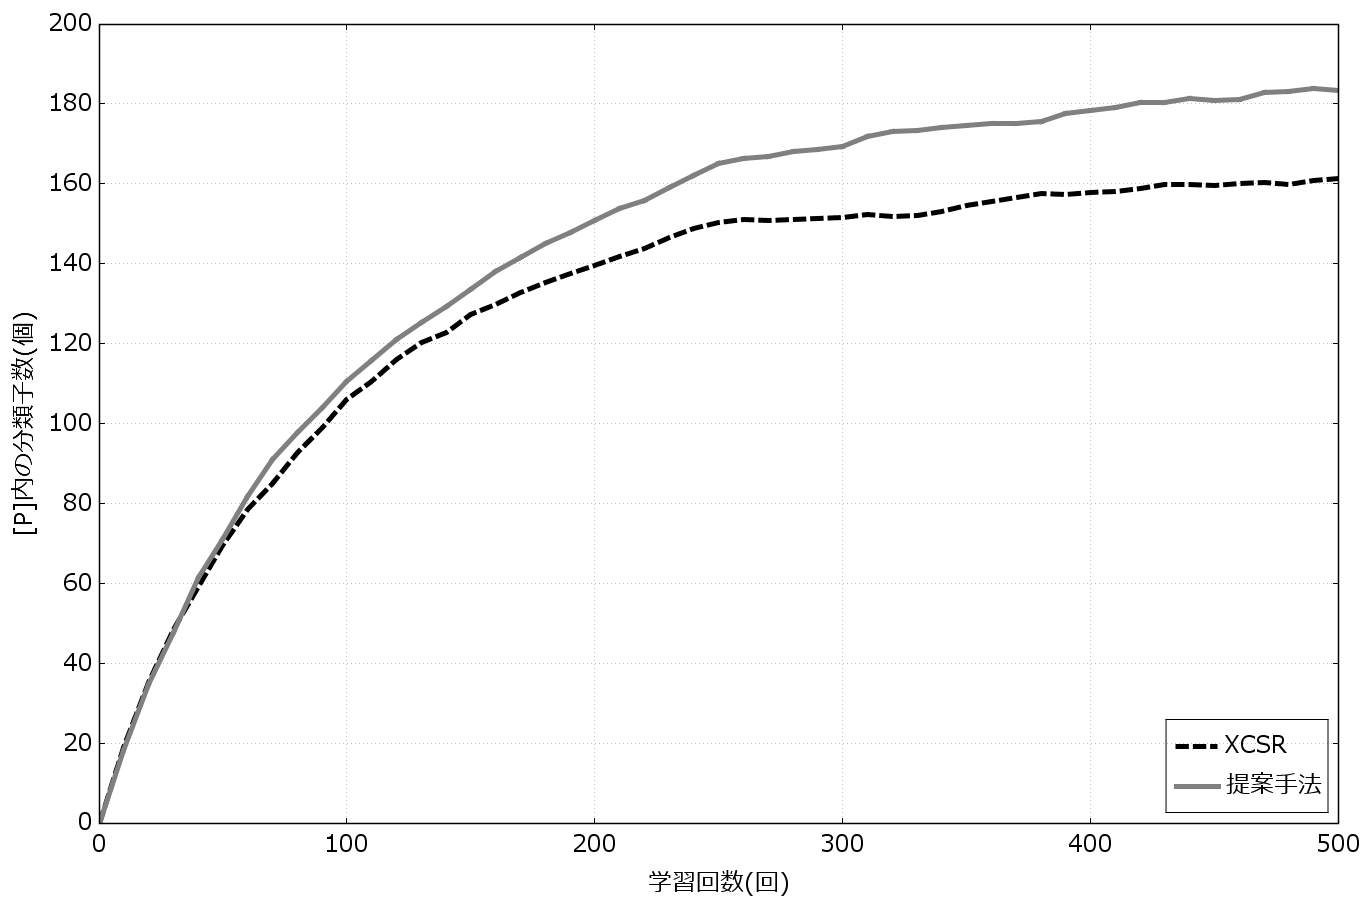
\includegraphics[width=0.45\textwidth]{population.bmp}
\caption{探索した局所解数の平均値(個体数別)}
\label{fig:pop*fit}
\end{center}
\end{figure}

\begin{figure}[h]
\begin{center}
\begin{tabular}{c}

\begin{minipage}[t]{0.45\linewidth}
\begin{center}
\includegraphics[keepaspectratio, scale=0.45]{sbat01_n10.bmp} (a) ${n=10}$
\end{center}
\end{minipage}

\begin{minipage}[t]{0.45\linewidth}
\begin{center}
\includegraphics[keepaspectratio, scale=0.45]{sbat01_n40.bmp} (b) ${n=40}$
\end{center}
\end{minipage}\\

\end{tabular}
\caption{分散型BAの解分布}
\label{fig:pop*pbestposition}
\end{center}
\end{figure}

\begin{figure}[h]
\begin{center}
\begin{tabular}{c}
\begin{minipage}[t]{0.45\linewidth}
\begin{center}
\includegraphics[keepaspectratio, scale=0.45]{sbat01.bmp} (c) ${s=1}$
\end{center}
\end{minipage}

\begin{minipage}[t]{0.45\linewidth}
\begin{center}
\includegraphics[keepaspectratio, scale=0.45]{sbat03_n20.bmp} (d) ${s=3}$
\end{center}
\end{minipage}\\
\end{tabular}
\caption{分散型BAの解分布}
\label{fig:s*pbestposition}
\end{center}
\end{figure}

\subsection{探索点(個体数)による効果}
Fig. \ref{fig:pop*fit} の縦軸を探索した解の数,横軸を個体数(探索率=探索した局所解/全局所解の数)とし,Fig. \ref{fig:pop*pbestposition} (a)(b) は1000世代目における個体の位置を示す.個体数の数に比例して探索性能は非常に高くなったが,同時に同じ局所解に陥る解も増加した.複数解探索において個体数の変化による影響は大きかったが,個体数の変化による個体全体の分散に影響は見られなかった.またFig. \ref{fig:fit_n=10} とFig. \ref{fig:fit_n=40}は探索した個体数別の最良解の時間推移である.このことから,個体数に応じて解探索の精度が変わるということがいえる.上述した個体数に比例して探索性能に影響を与えるということを裏付ける結果が得られた.
\begin{figure}[h]
\begin{center}
\includegraphics[width=0.45\textwidth]{sbat01_n10_pbest.bmp}
\caption{分散型BAの評価値 ${(n=10)}$}
\label{fig:fit_n=10}
\end{center}
\end{figure}

\begin{figure}[h]
\begin{center}
\includegraphics[width=0.45\textwidth]{sbat01_n40_pbest.bmp}
\caption{分散型BAの評価値 ${(n=40)}$}
\label{fig:fit_n=40}
\end{center}
\end{figure}

\subsection{シードによる影響}
Fig. \ref{fig:s*pbestposition}(a)(b) はあるシードの個体の位置を表し,Fig. \ref{fig:pbest_i=3}はそのシードにおける各個体の評価値を示す.Fig. \ref{fig:s_pbest} と比較すると,Fig. \ref{fig:pbest_i=3} のほうが早い段階で収束していることが分かるが,グラフよりあまり大きな変化はないと捉えることができる.しかし,${s=1}$では同じ局所解に複数の個体が位置し,${s=3}$では個体間の距離が遠くなるよう動作しているとグラフより読み取ることができる.またグラフより局所解に陥る個体の場所は,各個体の持つ評価値に依存し一様に決まらないといえる.
\begin{figure}[t]
\begin{center}
\includegraphics[width=0.45\textwidth]{sbat03_n20_pbest.bmp}
\caption{分散型BAの評価値${x_{i*}}$\  (s=3)}
\label{fig:pbest_i=3}
\end{center}
\end{figure}

\section{終わりに}
本論文では,従来のBAにおける最良解を参照することによる全個体の最適解への収束を防ぎ,
複数の局所解を網羅的に探索する2つの修正を加えた分散型BAを提案した.
具体的に修正した点は以下の2つである.
(1)各世代において各個体間の距離を考慮した速度の更新;
(2)新たな解の生成時に各個体の最良解(パーソナルベスト)を参照した解の生成.
提案手法である分散BAの複数の局所解の網羅的な探索性能を検証を目的として,
複数の局所解を持つ多峰性ベンチマーク関数を用いたシミュレーション実験により,
探索した局所解の個数,最適解付近の探索性能の2つの観点に関して,従来手法であるBAと比較した.
その結果,分散型BAの最適解付近の探索性能は従来のBAに比べて低下したが,
従来手法に比べて,分散型BAは複数の局所解の網羅的な探索性能が向上した.
その理由として,(1)の修正により各個体同士が離れやすくなり,さらに(2)の修正により各個体が探索した各個体の最良解の付近の局所的な探索が有効に働いたと考えられる.
しかし,分散型BAは多くの局所解を探索できているものの,すべての局所解を探索することはできなかった.
また,分散型BAは早い段階で探索が収束してしまったため,探索を制御するパラメータであるラウドネスとパルスレートの調整も検討すべきである.
そのため,今後の課題として,すべての局所解を探索可能な機構の導入,最適なパラメータの調査の2つを考慮した複数の局所解の網羅的探索性能向上を目指す.\\


\small
\begin{thebibliography}{10}
%%%%%%%%%%%%%%%%%%%%%%%%%%%%%%%%%%%%%%%%%%%%%%%%%%%%%%%%%%%%%%%%%%%%%%%%%%%%%%%

%\bibitem{大会ホームページ}
%{\tt http://www.sice.or.jp/org/SSI2015/}

\bibitem{1}
Yang, X. S. “A Metaheuristic Bat-Inspired Algorithm”, in: Nature Inspired Cooperative Strategies for Optimization (NISCO 2010) (Eds J.R. Gonzalez et al.), Studies in Com-putational Intelligence, Springer Berlin, 284, Springer, 65-74 (2010)

\bibitem{2}
Eberhart, R. C., and Kennedy, J. :“A New Optimizer Using Particle Swarm Theory”,
Proc. Sixth International Symposium on Micro Machine and Human Science (Nagoya, Japan), IEEE Service center, Pis-cataway, NJ, 39-43 (1995)

\bibitem{3}
Yang, X. S. ”Firefly Algorithms for Multimodal Optimization”,in:Stochastic Algorithms: Foundations and Applications, SAGA 2009, Lecture Notes in Computer Sciences, Vol. 5792, pp. 169-178 (2009)

\bibitem{4}
上村 昌史 “複数解探索を行うFirefly Algorithm”,電子情報通信学会技術研究報告, 信学技報113(271), 1-4, NLP2013-69(2013-10), Vol. 5792, pp. 169-178 (2009)

\bibitem{5}
R., Takano, T. Harada, and K., Takadama. "Artificial bee colony algorithm based on local information sharing in dynamic environment.", Proceedings of the 18th Asia Pacific Symposium on Intelligent and Evolutionary Systems, Volume 1. Springer, Cham, (2015).

\bibitem{6}
Surjanovic, S. and Bingham, D. (2013).  Virtual Library of Simulation Experiments: Test Functions and Datasets,Retrieved October 9, (2017)
%%%%%%%%%%%%%%%%%%%%%%%%%%%%%%%%%%%%%%%%%%%%%%%%%%%%%%%%%%%%%%%%%%%%%%%%%%%%%%%
\end{thebibliography}
\normalsize

\end{document}
